% ---- closed --------

\begin{figure}[!htb]
    \centering
    \begin{minipage}[b]{0.45\textwidth}
        \centering
        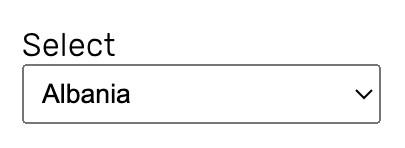
\includegraphics[width=0.8\textwidth]{closed.osx.chrome.png}
        \caption{Geschlossenes Select auf OSX Chrome}
        \label{Abbildung:closedOsxChromeSelect}
    \end{minipage}
    \hfill
    \begin{minipage}[b]{0.45\textwidth}
        \centering
        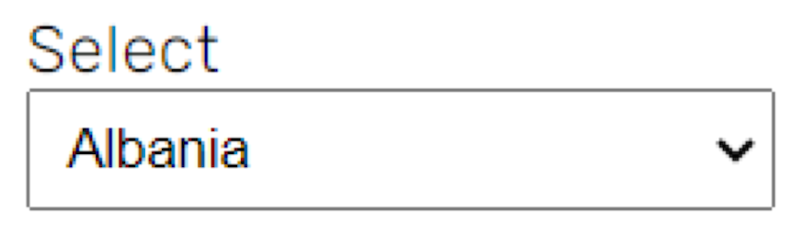
\includegraphics[width=0.8\textwidth]{closed.win.chrome.png}
        \caption{Geschlossenes Select auf Windows Chrome}
        \label{Abbildung:closedWinChromeSelect}
    \end{minipage}
\end{figure}

\begin{figure}[!htb]
    \centering
    \begin{minipage}[b]{0.45\textwidth}
        \centering
        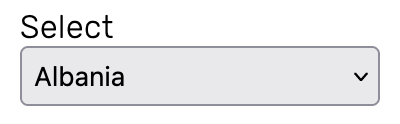
\includegraphics[width=0.8\textwidth]{closed.osx.firefox.png}
        \caption{Geschlossenes Select auf OSX Firefox}
        \label{Abbildung:closedOsxFirefoxSelect}
    \end{minipage}
    \hfill
    \begin{minipage}[b]{0.45\textwidth}
        \centering
        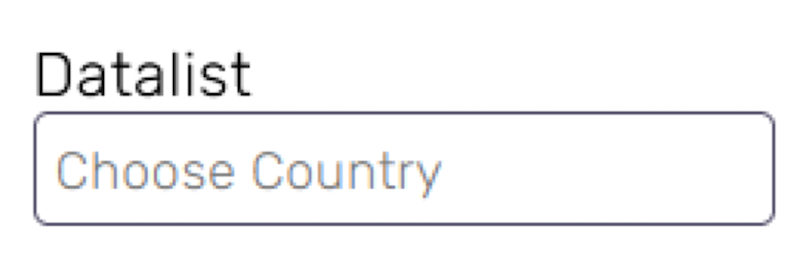
\includegraphics[width=0.8\textwidth]{closed.win.firefox.png}
        \caption{Geschlossenes Select auf Windows Firefox}
        \label{Abbildung:closedWinFirefoxSelect}
    \end{minipage}
\end{figure}

\begin{figure}[!htb]
    \centering
    \begin{minipage}[b]{0.45\textwidth}
        \centering
        
\includegraphics[width=0.8\textwidth]{closed.osx.safari.png}
        \caption{Geschlossenes Select auf OSX Safari}
        \label{Abbildung:closedOsxSafariSelect}
    \end{minipage}
    \hfill
    \begin{minipage}[b]{0.45\textwidth}
        \centering
        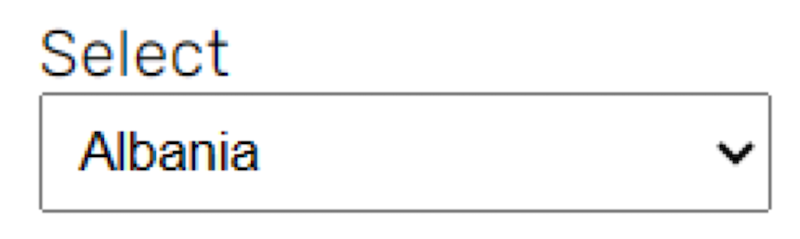
\includegraphics[width=0.8\textwidth]{closed.win.edge.png}
        \caption{Geschlossenes Select auf Windows Edge}
        \label{Abbildung:closedWinEdgeSelect}
    \end{minipage}
\end{figure}

% ---- opened --------

\begin{figure}[!htb]
    \centering
    \begin{minipage}[b]{0.28\textwidth}
        \centering
        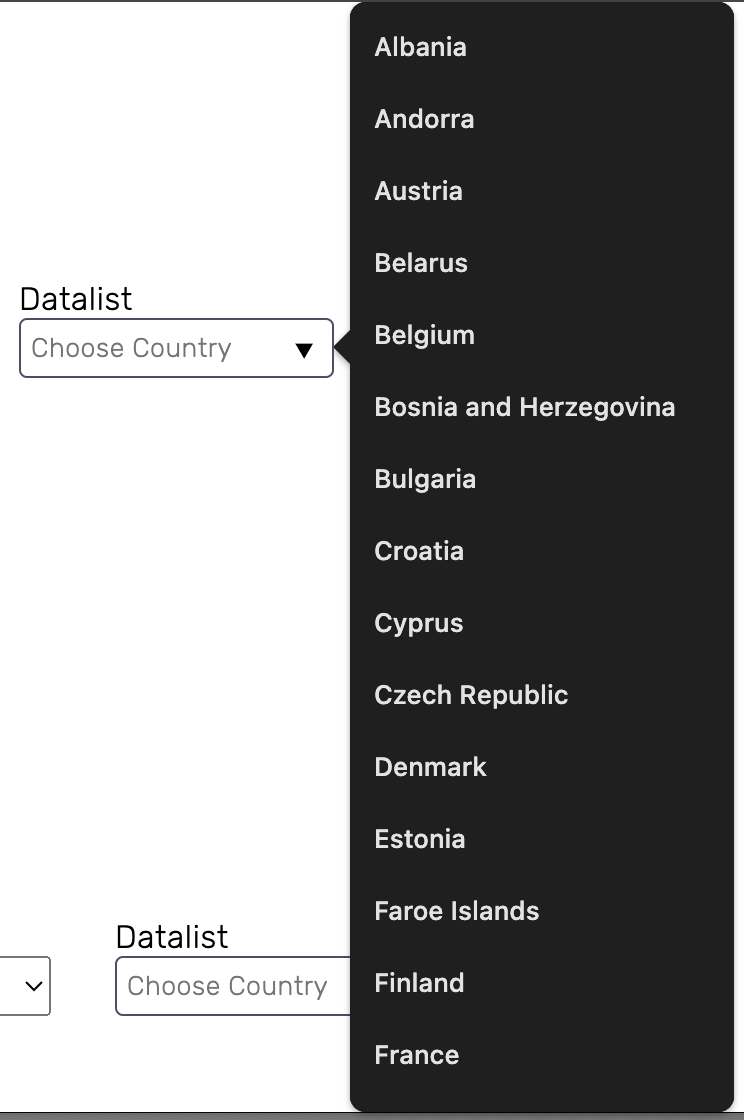
\includegraphics[width=0.55\textwidth]{opened.osx.chrome.png}
        \caption{Offenes Select auf OSX Chrome}
        \label{Abbildung:openedOsxChromeSelect}
    \end{minipage}
    \hfill
    \begin{minipage}[b]{0.28\textwidth}
        \centering
        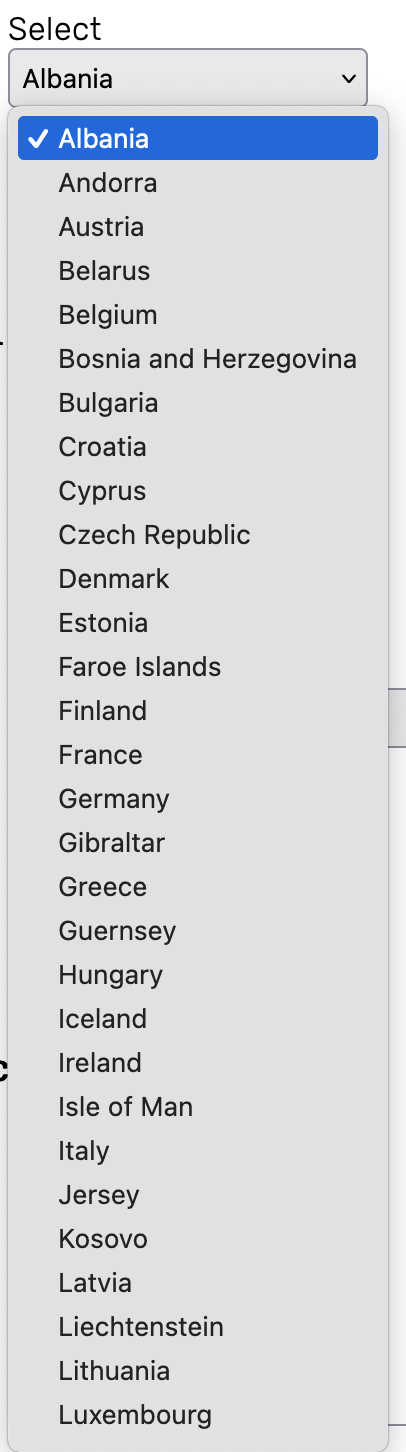
\includegraphics[width=0.5\textwidth]{opened.osx.firefox.png}
        \caption{Offenes Select auf OSX Firefox}
        \label{Abbildung:openedOsxFirefoxSelect}
    \end{minipage}
    \hfill
    \begin{minipage}[b]{0.28\textwidth}
        \centering
        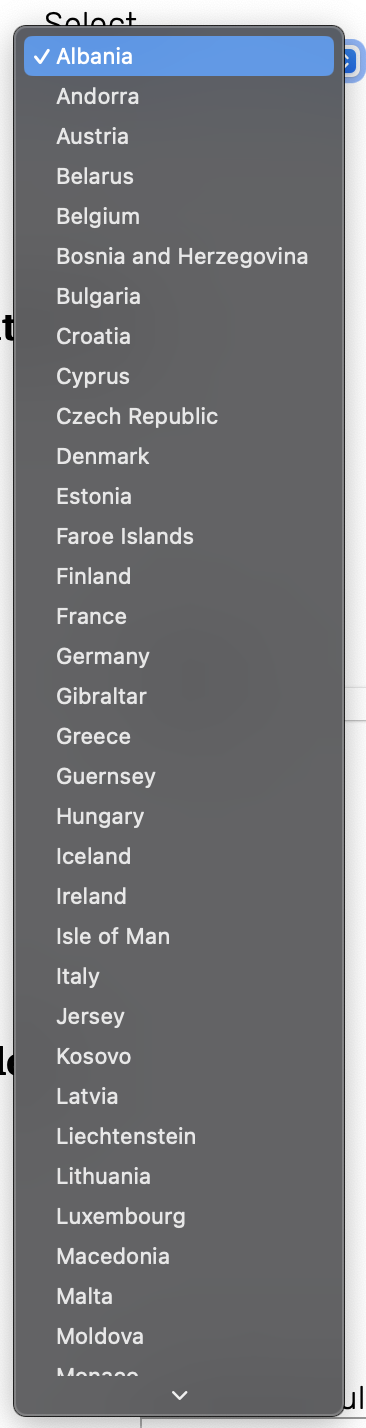
\includegraphics[width=0.45\textwidth]{opened.osx.safari.png}
        \caption{Offenes Select auf OSX Safari}
        \label{Abbildung:openedOsxSafariSelect}
    \end{minipage}
\end{figure}

\begin{figure}[!htb]
    \centering
    \begin{minipage}[b]{0.28\textwidth}
        \centering
        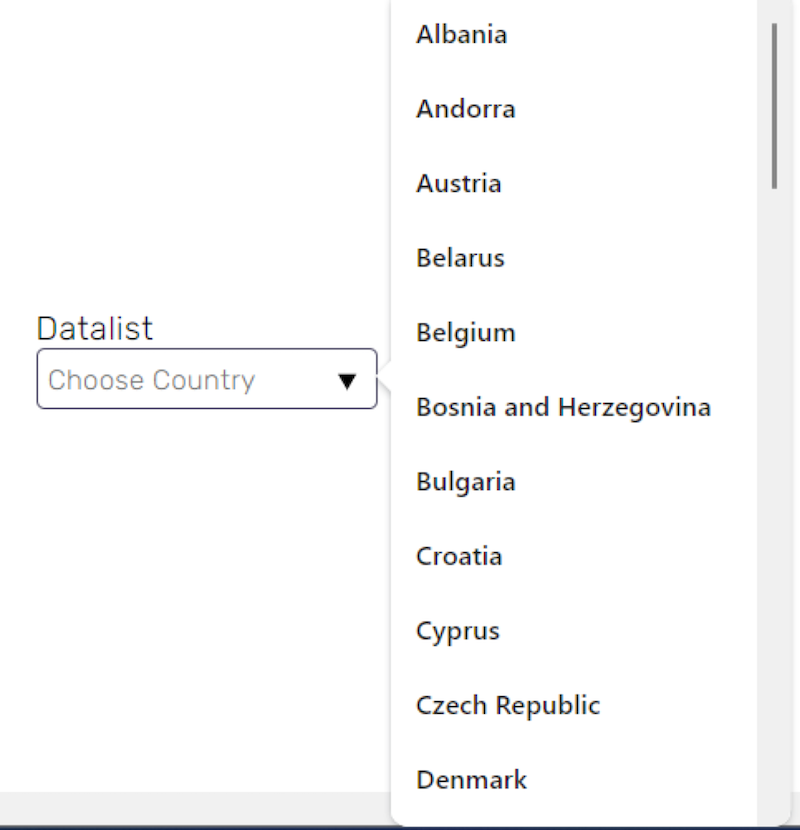
\includegraphics[width=0.65\textwidth]{opened.win.chrome.png}
        \caption{Offenes Select auf Windows Chrome}
        \label{Abbildung:openedWinChromeSelect}
    \end{minipage}
    \hfill
    \begin{minipage}[b]{0.28\textwidth}
        \centering
        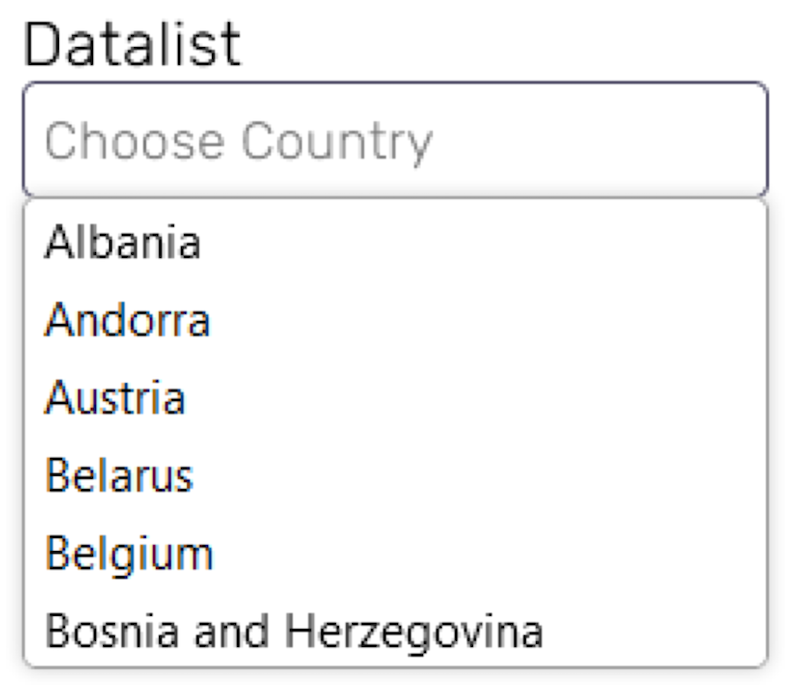
\includegraphics[width=0.6\textwidth]{opened.win.firefox.png}
        \caption{Offenes Select auf Windows Firefox}
        \label{Abbildung:openedWinFirefoxSelect}
    \end{minipage}
    \hfill
    \begin{minipage}[b]{0.28\textwidth}
        \centering
        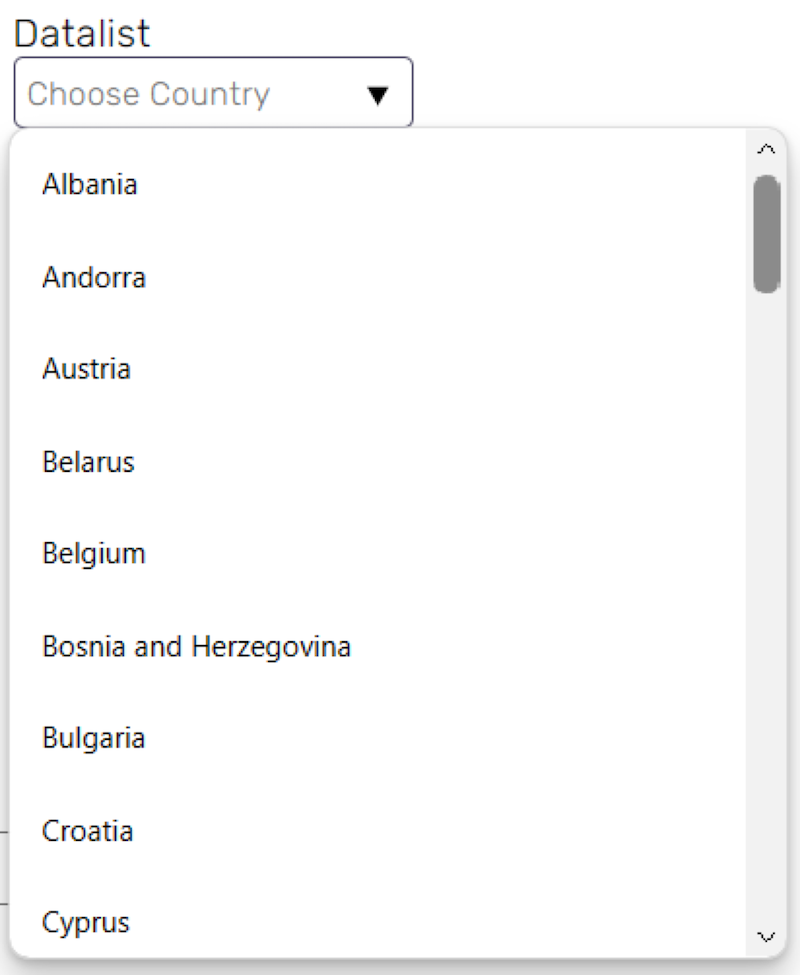
\includegraphics[width=0.65\textwidth]{opened.win.edge.png}
        \caption{Offenes Select auf Windows Edge}
        \label{Abbildung:openedWinEdgeSelect}
    \end{minipage}
\end{figure}
